\documentclass[../main.tex]{subfiles}

\begin{document}

\chapter{Alogrithms}

This appendix details the applied encryption and decryption algorithms.

\section{Encryption algorithm}
\label{app:encryption}
\begin{figure}[h]
    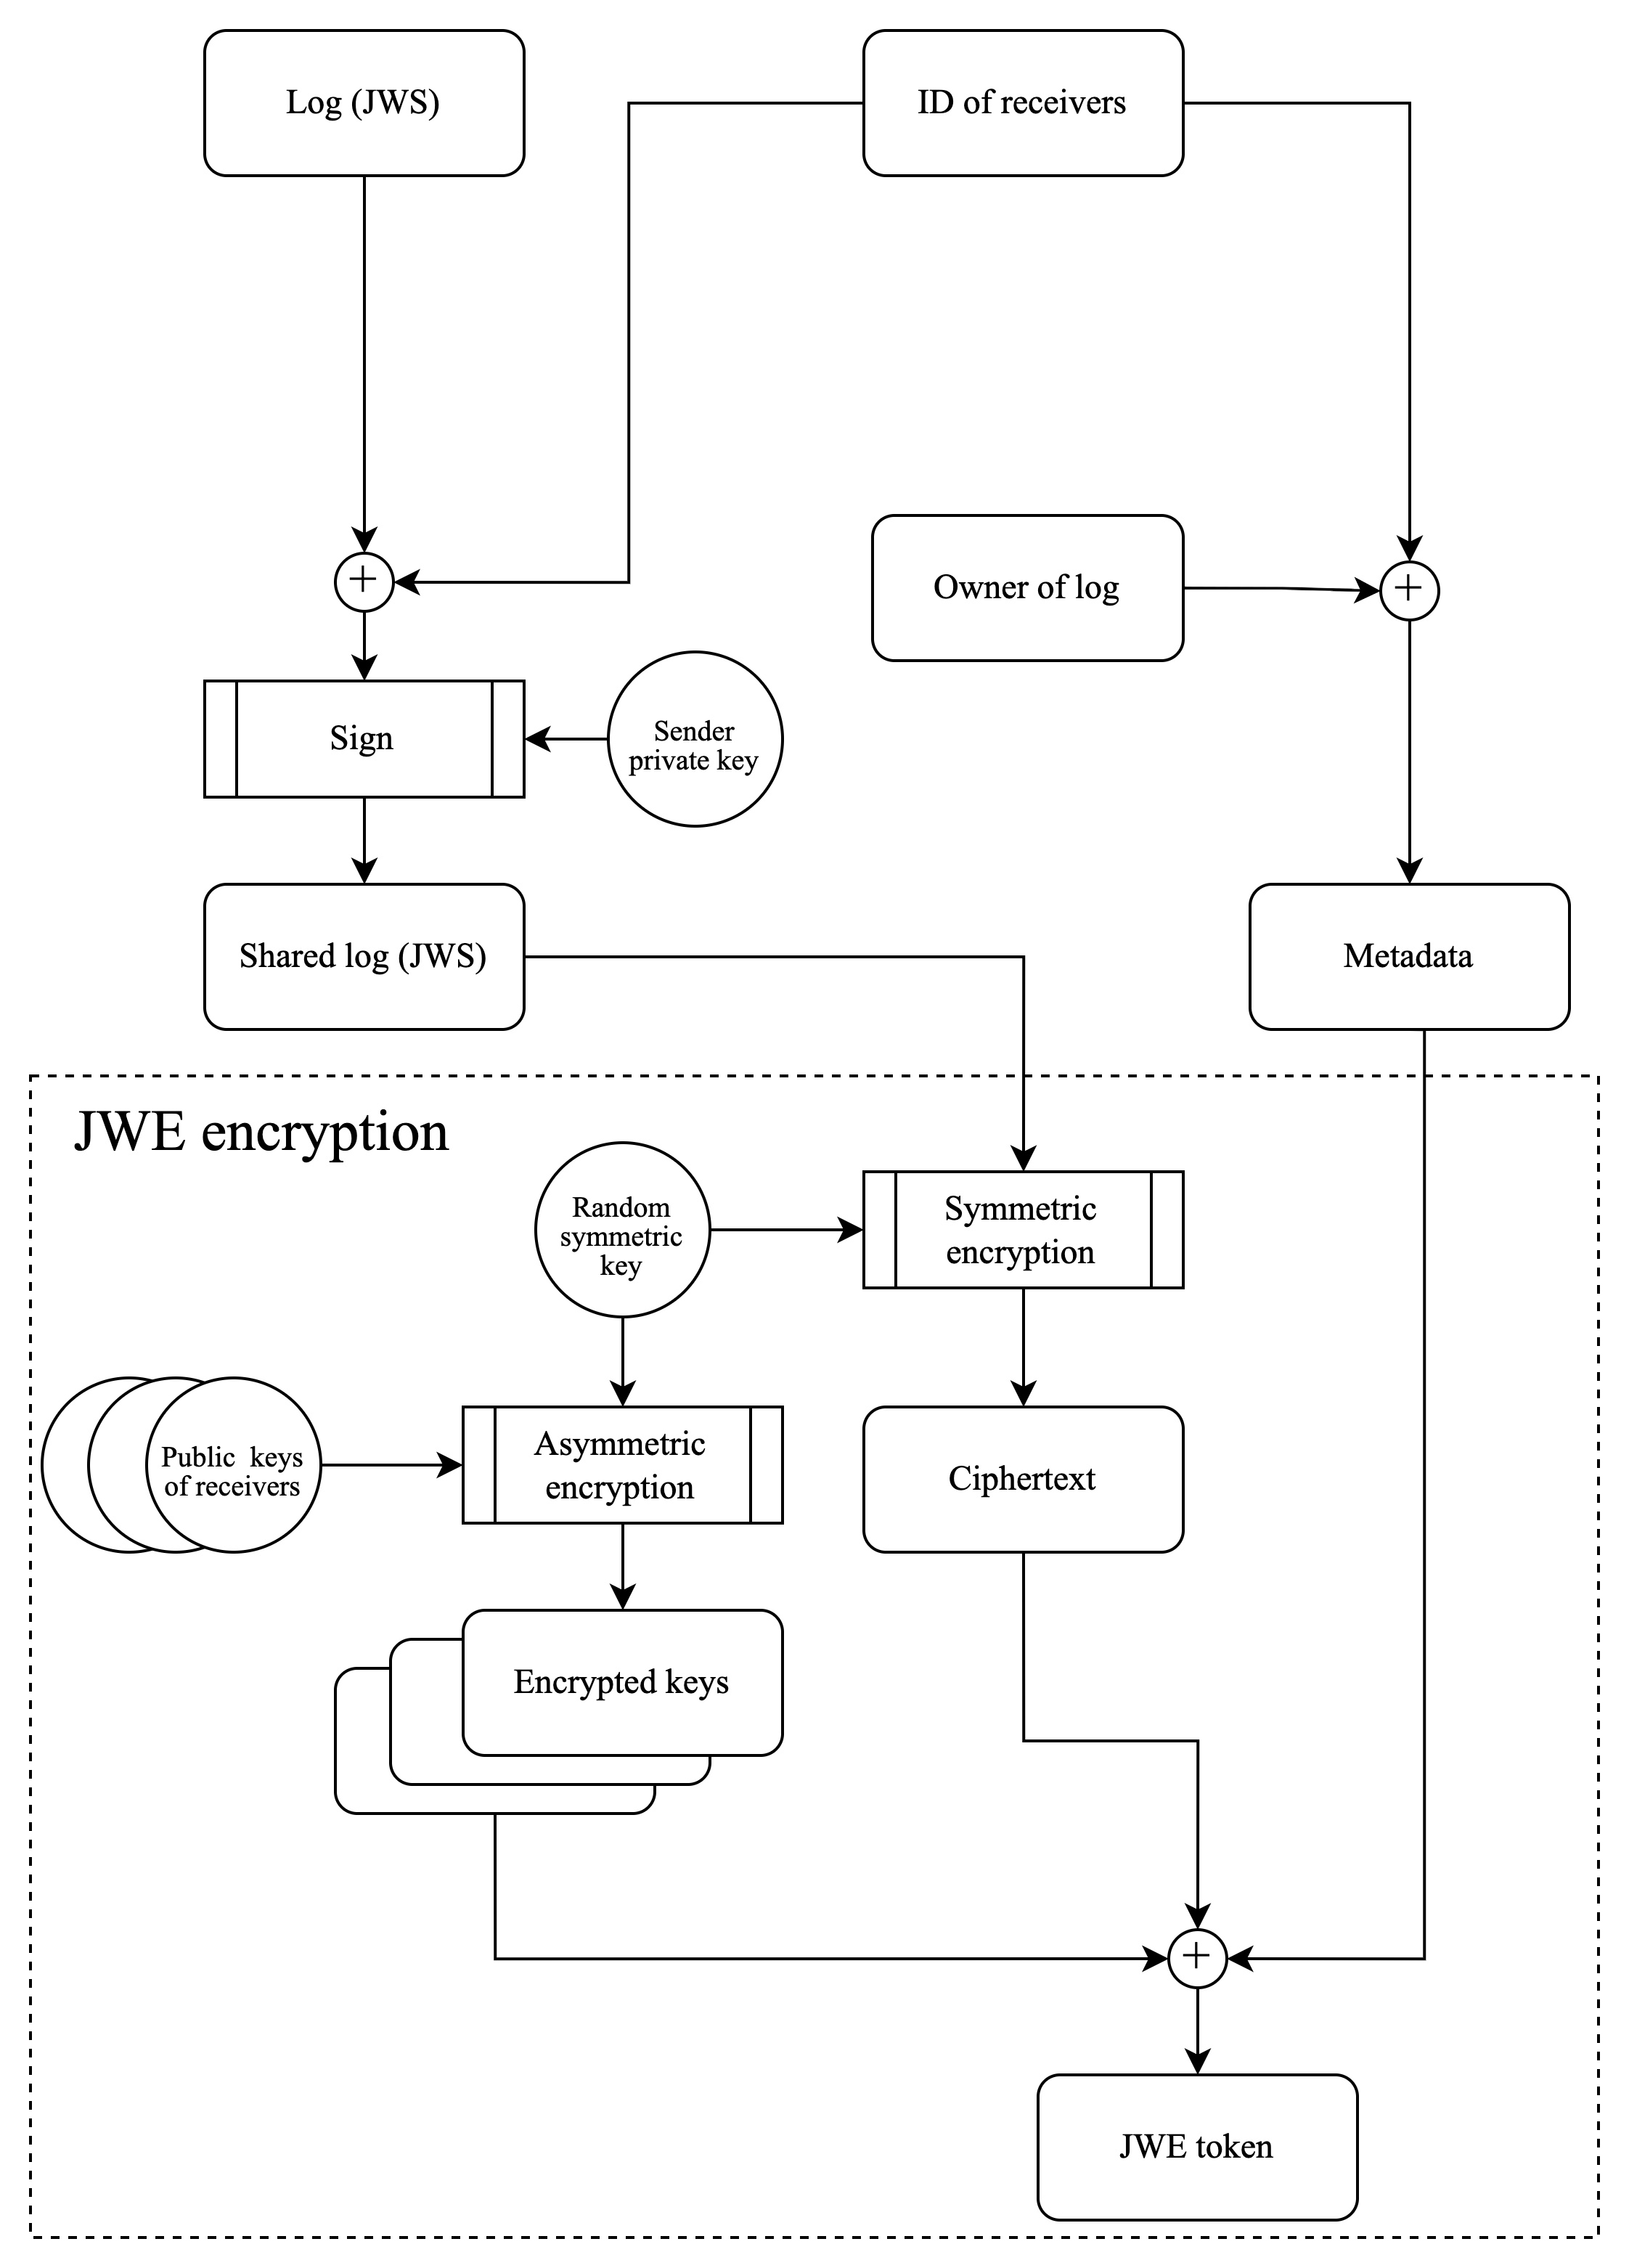
\includegraphics[scale=0.13]{../img/05/encrypt_logs.jpg}
    \centering
    \caption{The encryption algorithm takes a signed log and a set of receivers as input. It returns a JWE-token which can only be decrypted by the specified set of users.}
    \label{app:encryption_algo}
\end{figure}
\newpage
\section{Decryption algorithm}
\label{app:decryption}
\begin{figure}[h]
    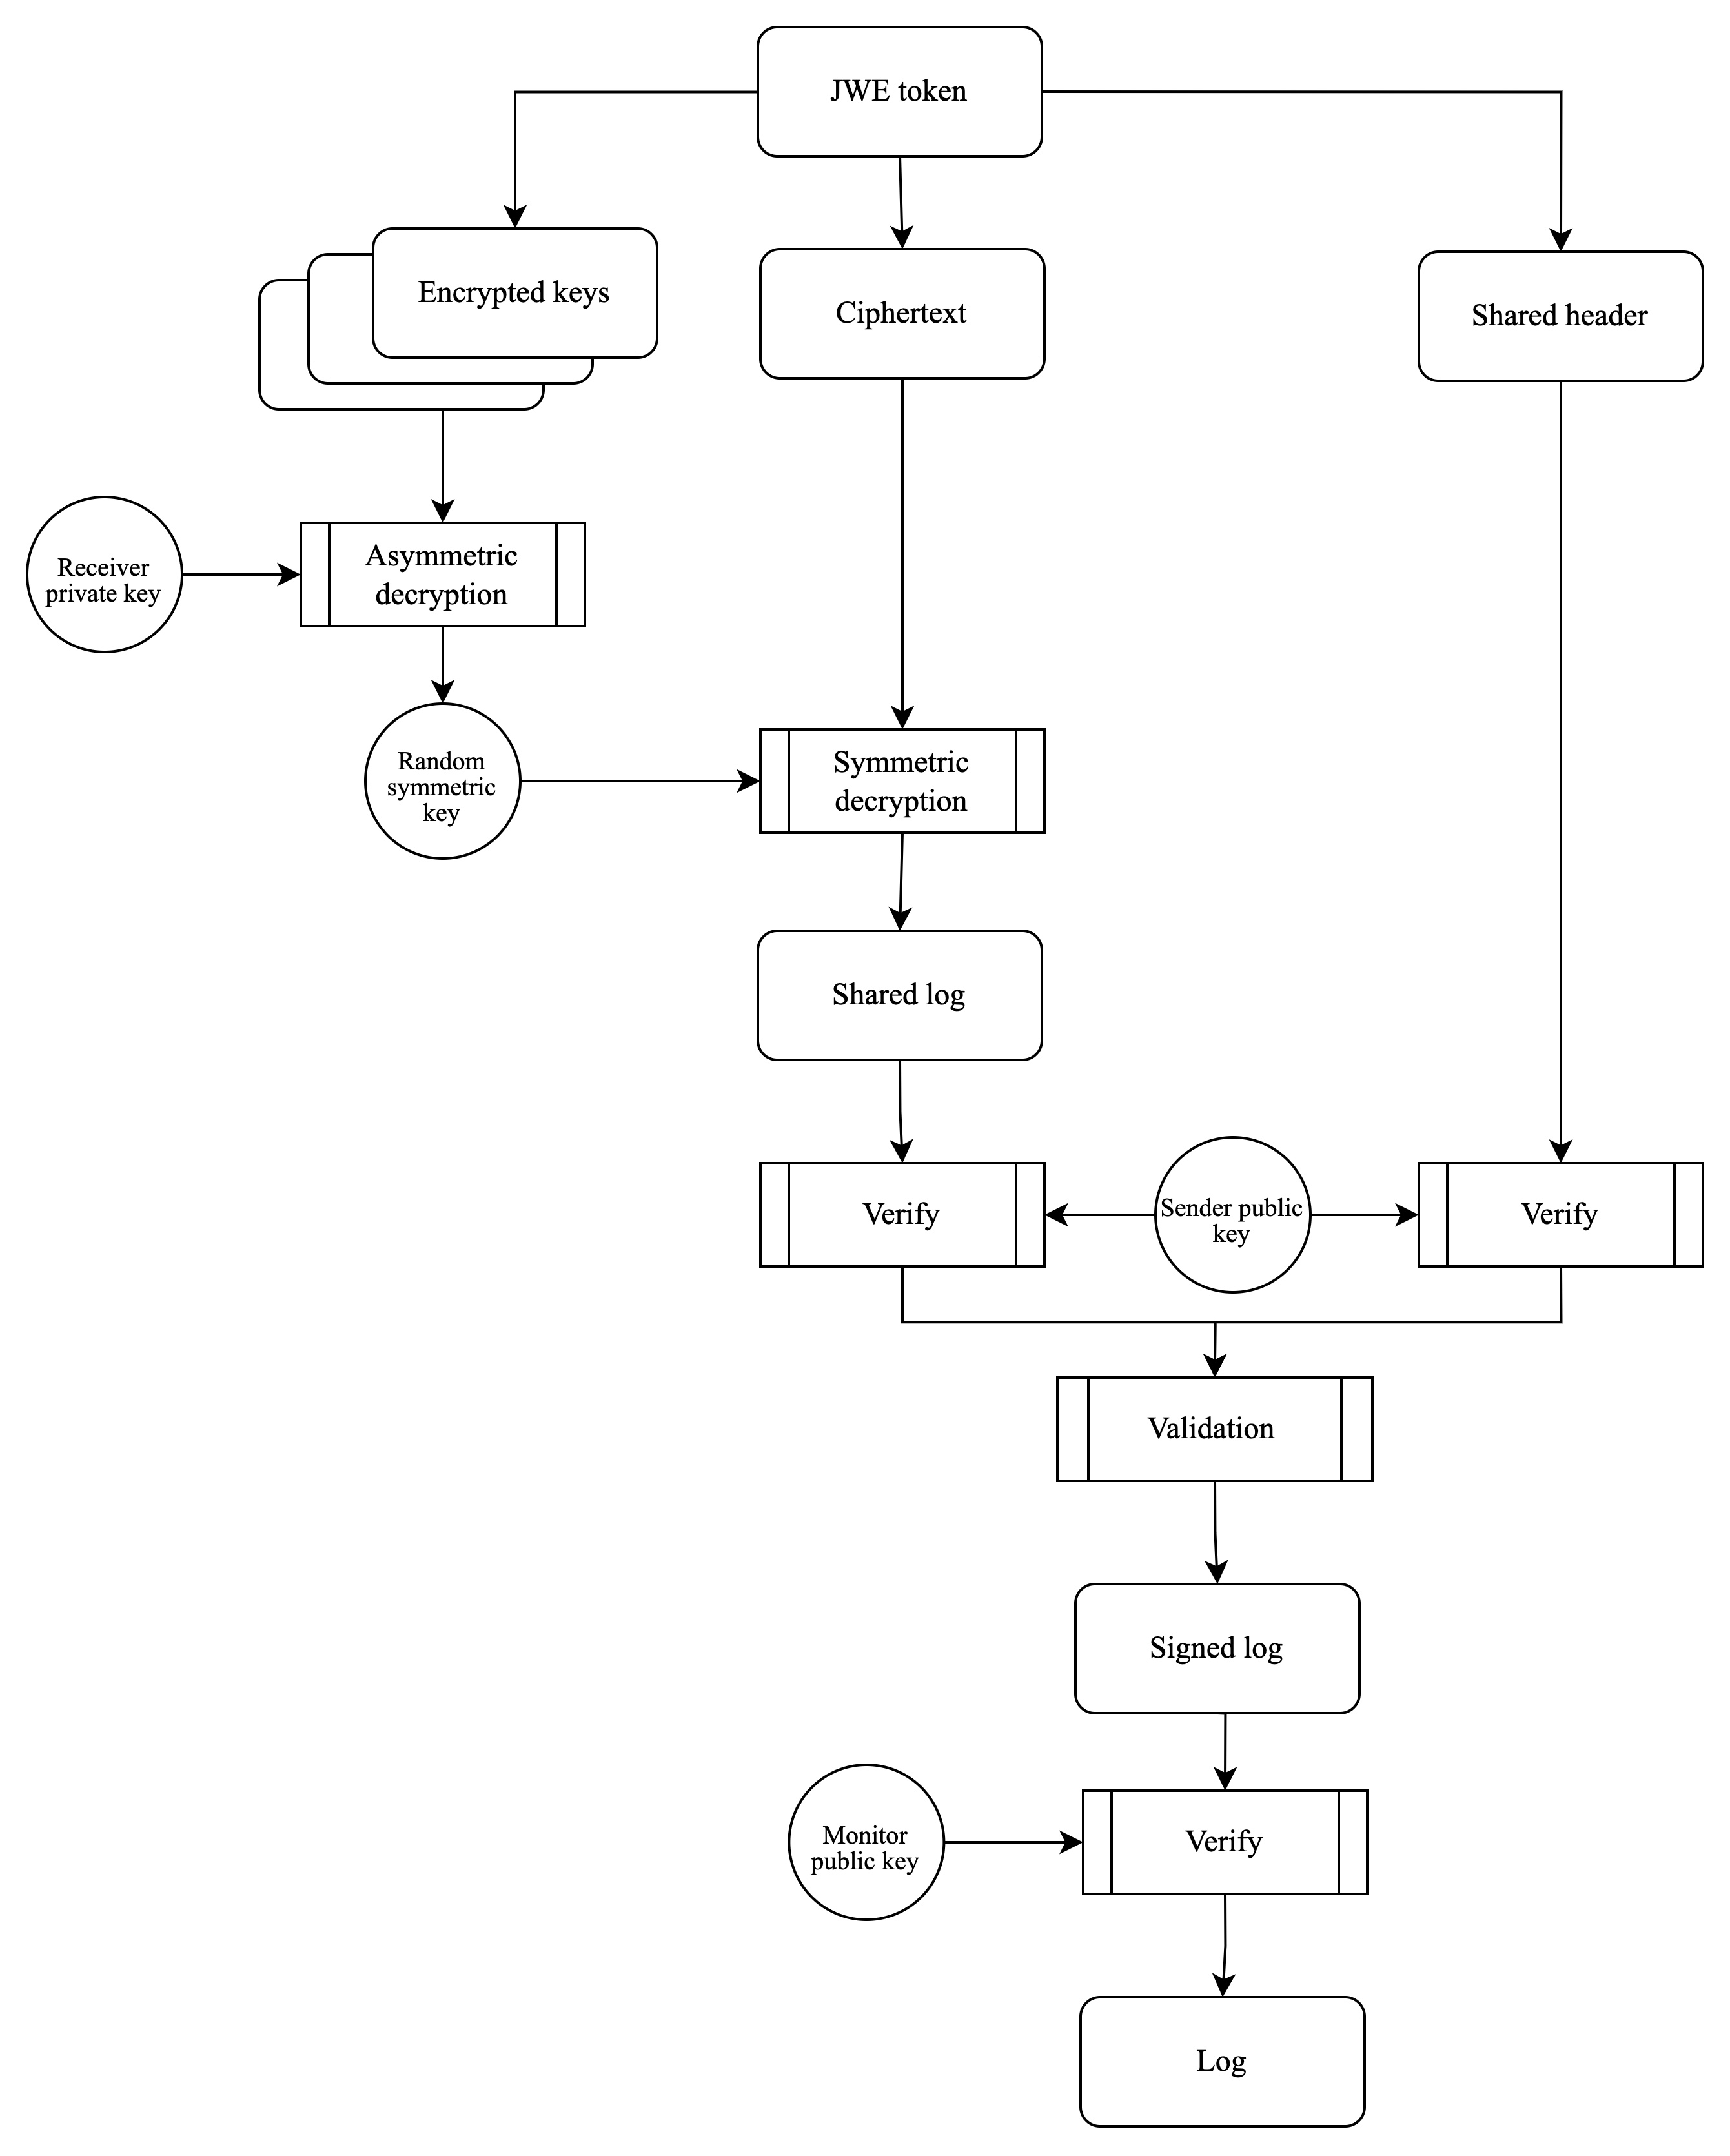
\includegraphics[scale=0.13]{../img/05/decrypt_logs.jpg}
    \centering
    \caption{The decryption algorithm takes a JWE token and a private decryption key as input. It returns the decrypted log if the user is allowed to decrypt.}
    \label{app:decryption_algo}
\end{figure}

\chapter{Screenshots Clotilde UI}

This appendix contains screenshots of the implemented features in the \emph{Clotilde UI}.

\label{app:screenshots}
\begin{figure}[h!]
    \fbox{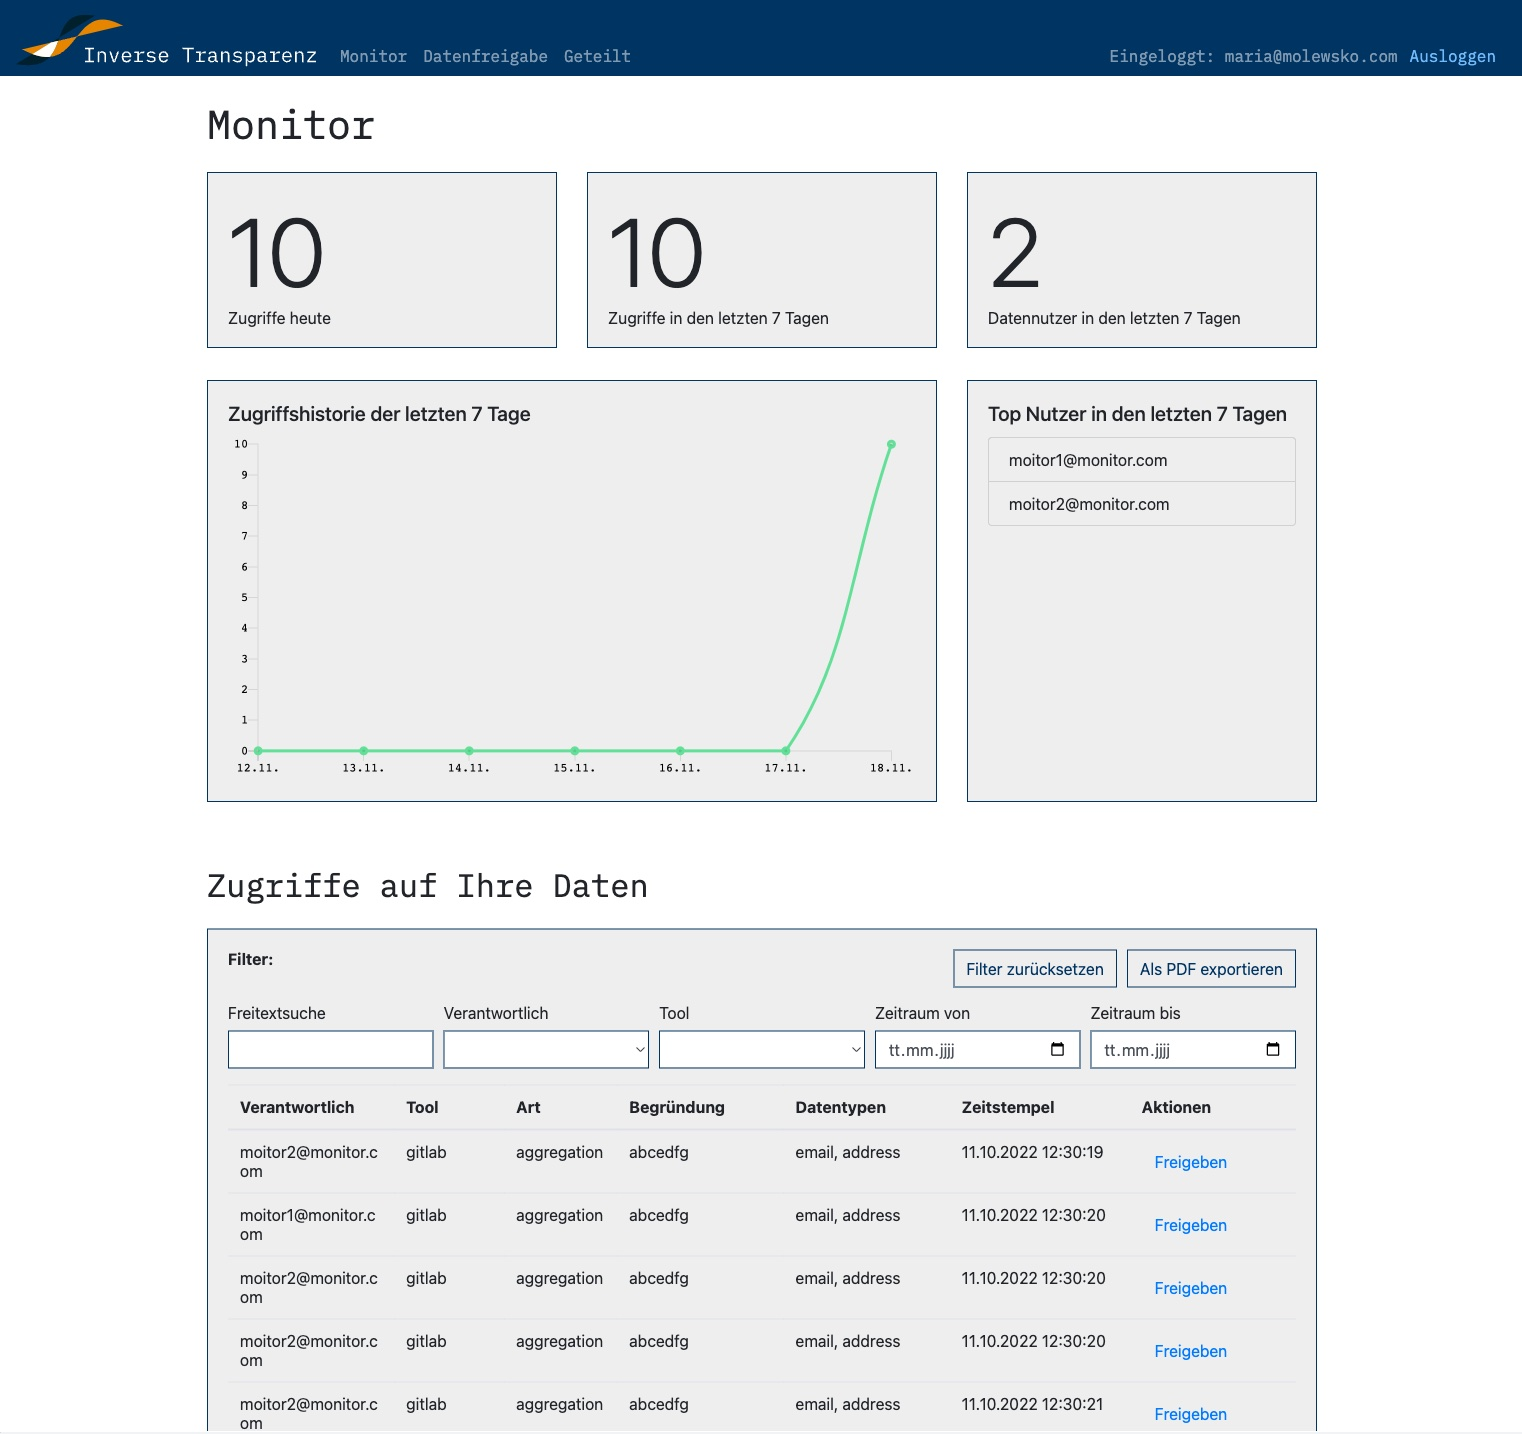
\includegraphics[scale=0.25]{../img/06/clotilde_overview.jpg}}
    \centering
    \caption{
        The updated overview page of the Clotilde UI. 
        All logs are visualized as before. 
        The user can share or revoke access the users having access to a log by clicking on the corresponding button in the table.}
    \label{app:clotilde-overview}
\end{figure}
\newpage
\begin{figure}[h!]
   \fbox{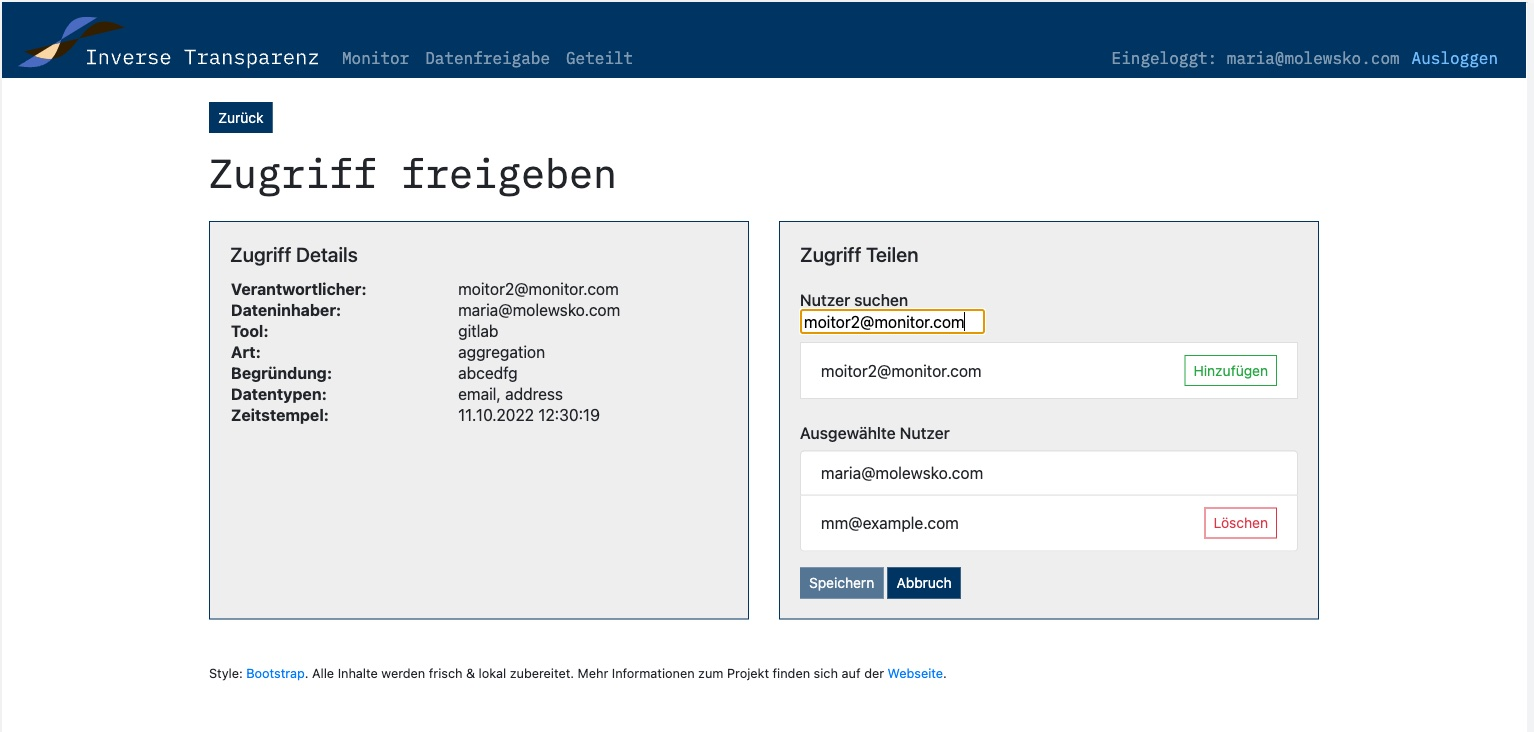
\includegraphics[scale=0.25]{../img/06/clotilde_share.jpg}}
    \centering
    \caption{
        This view allows the user to share or revoke access to a log. 
        On the left-hand side the details of the log are displayed. 
        On the right-hand side the user can search for other users in the system. 
        If a user is found it can be added to the set of recipients. 
        Moreover, the access to certain users can be revoked by removing them from the list of recipients.}
    \label{app:clotilde-share}
\end{figure}

\begin{figure}[h!]
    \fbox{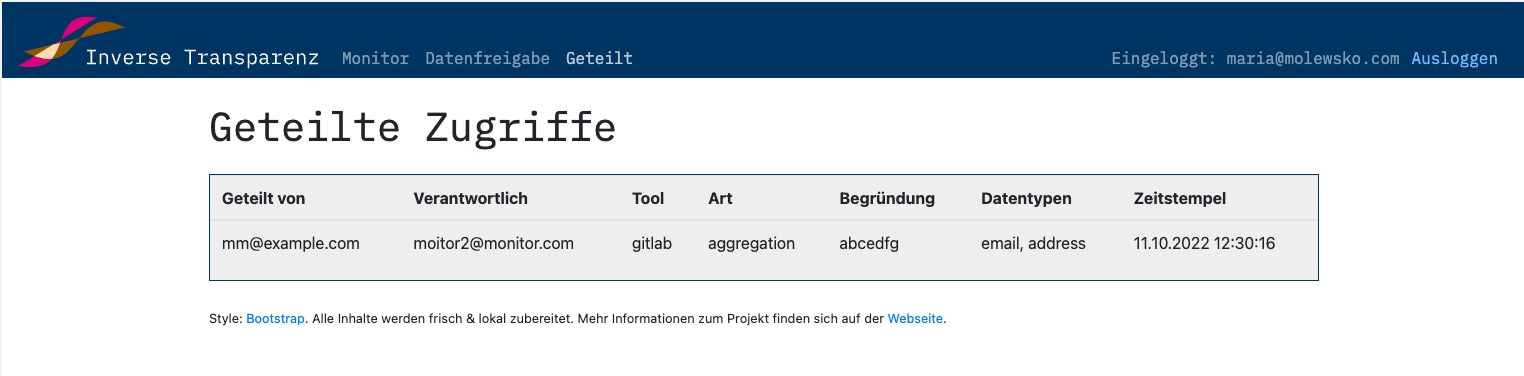
\includegraphics[scale=0.25]{../img/06/clotilde_shared.jpg}}
    \centering
    \caption{
        This view lists all logs which were shared with the logged-in users.
        It is realized as additional section within the menu.
    }
    \label{app:clotilde-shared}
\end{figure}

\end{document}
